\documentclass[xcolor=pdftex,dvipsnames,table,10pt]{beamer}
\usepackage{verbatim}
\usepackage{color}


\setbeamerfont{block title}{size={}}
\setbeamerfont{frametitle}{size=\large,series=\bfseries}
\setbeamertemplate{navigation symbols}{}
\definecolor{darkgreen}{RGB}{106,168,82}
\definecolor{kugreen}{RGB}{50,93,61}
\usetheme{Malmoe}

\usecolortheme{beetle}
\setbeamercovered{invisible}
\setbeamercolor{item}{fg=black}
\setbeamercolor{normal text}{bg=white,fg=black}
\setbeamercolor{frametitle}{fg=white,bg=beetle@other}
\setbeamercolor{title}{fg=white}
 \setbeamercolor{section in toc}{fg=black}
 \setbeamertemplate{section in toc}[sections numbered]
\setbeamertemplate{subsection in toc}[ball unnumbered]
\setbeamercolor{titlelike}{fg=white,parent=palette primary}
\graphicspath{{./pics/}}


\setbeamerfont{block title}{size={}}
\setbeamertemplate{blocks}[rounded][shadow=true] 
\setbeamercolor{block title}{bg=beetle@other}
 
 \date{}
 \title{Association testing and GWAS}
%\author[Ida Moltke, summer course, August 2016]{\includegraphics[trim = 0mm 0mm 0mm 0mm,clip=true,scale=1.2]{i-30fd6d40d1bc145dfcdd981b239a43e9-wtccc_manhattan.jpg}\\
\author[Line Skotte, Medical and Population Genetics Course, August 2018]{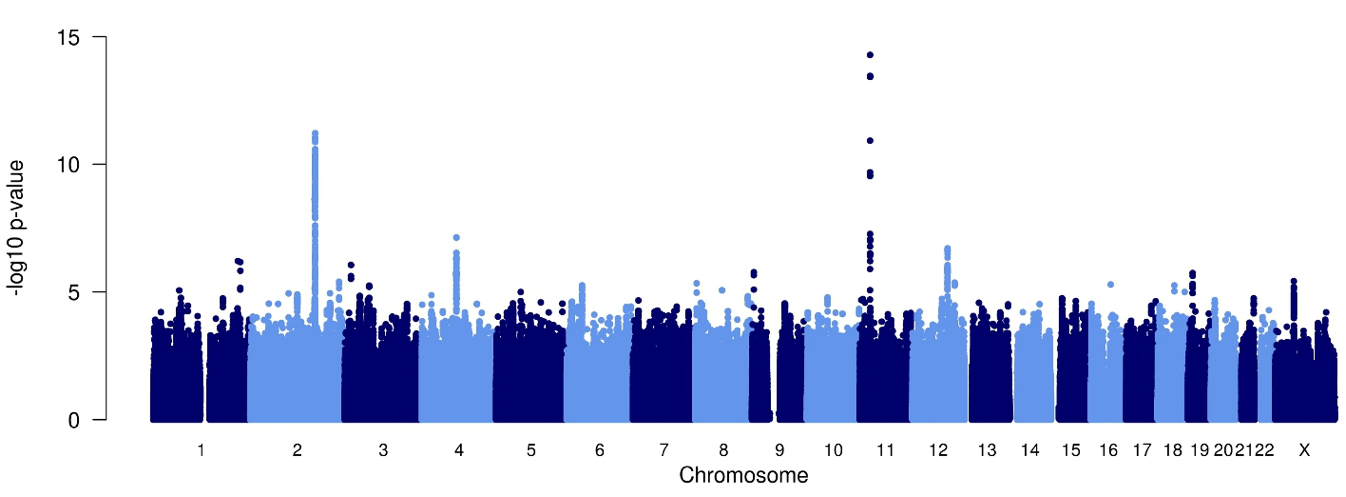
\includegraphics[width=0.8\textwidth]{febrile_gwas.png}\\
\vspace{0.2cm} Line Skotte, Medical and Population Genetics Course, August 2018\vspace{-1.5cm}}

\begin{document} 

\begin{frame}[plain]
\titlepage
\end{frame}




\AtBeginSection[]
{ 
   \begin{frame}
       \frametitle{Outline}
       \small
       \tableofcontents[currentsection] 
   \end{frame}
}


\section{Introduction}

\subsection{Motivation}
\begin{frame}
  \frametitle{What and why?}
   \vspace{-2.00cm} 
   \small 
    \begin{itemize}\setlength{\itemindent}{-1em}
    \item \textbf{Goal: to identify (map) genetic variants that have an effect on a trait}\\
    \item Typically \textbf{disease related traits}, e.g. febrile seizures 
   % \item I.e. studies where the trait is whether the participants have \\\hspace{-.325cm}a disease (cases) or not (controls)\\\vspace{0.5cm}
  %     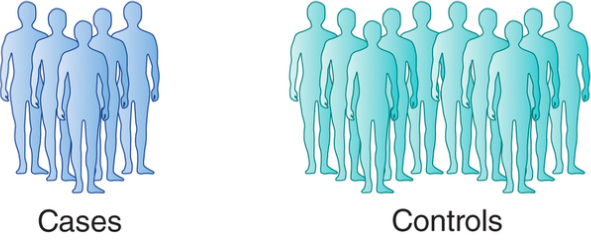
\includegraphics[scale=.2]{cc.png}\\\vspace{0.05cm}
  \item<2-> Motivation: reaching this goal can help
  \begin{itemize}\setlength{\itemindent}{-1em}
  \item reveal the underlying genetic architecture 
  \item hopefully lead to better understanding of what \textbf{causes} the disease
  \item in turn ideally lead to better treatment and/or prevention
  \end{itemize}
  \item<3-> Note, \textbf{can also be used in e.g. evolutionary studies!}%as illustrated in Matteo's talk 
  \end{itemize}
\end{frame}


\subsection{Plan for today}
\begin{frame}
  \frametitle{Plan for today (to teach you how)}
  % \vspace{-1.0cm} 
   \small 
    \begin{itemize}\setlength{\itemindent}{-2.5em}
    \item<1-> \textbf{This afternoon:} 
  \begin{itemize}\setlength{\itemindent}{-3.75em}
  \item How to test if a genetic variant potentially affects a trait (single SNP tests)
  \item How to search the genome for variants that affect a given trait (GWAS)
  \item We will assume we have genotyping data (e.g. from SNP chip)
  \item We will assume there is no population structure
  \item We will look at disease status traits:\\\vspace{0.2cm}
     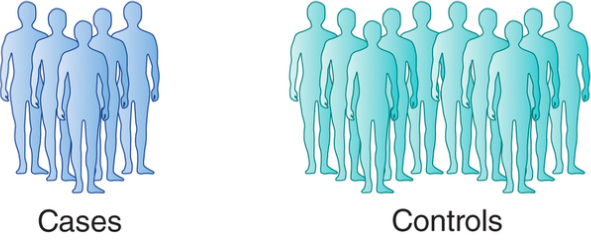
\includegraphics[scale=.2]{cc.png}
     \item And quantitative traits:\\\vspace{-0.9cm}
     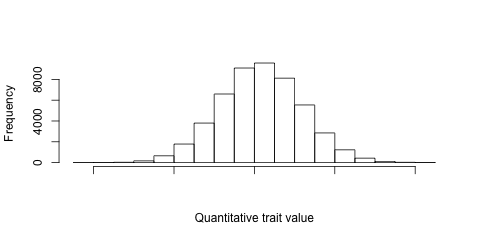
\includegraphics[scale=.4]{qtv_hist.png}
    \end{itemize}
  %\item<2-> \textbf{Tomorrow morning (Bjarni):} 
  %\begin{itemize}\setlength{\itemindent}{-3.75em}
  %\item How to deal with quantitative traits
  % \item How to deal with/exploit population structure
  % \item Other exiting advanced methods
  %  \end{itemize}
  \end{itemize}
\end{frame}

\section{Single SNP tests}

\subsection{A range of tests}
\begin{frame}
  \frametitle{Overall idea in association testing}
  \vspace{.1cm}  
 \small 
\hspace{-0.4cm}\textbf{How do we test if a genetic variant potentially has an effect on a disease?}\\\vspace{0.0cm}
  \begin{itemize}\setlength{\itemindent}{-2.25em}
    \item<2-> Idea: test for \textbf{association} between the variant and disease status (case/control)\\\vspace{-0.25cm}
        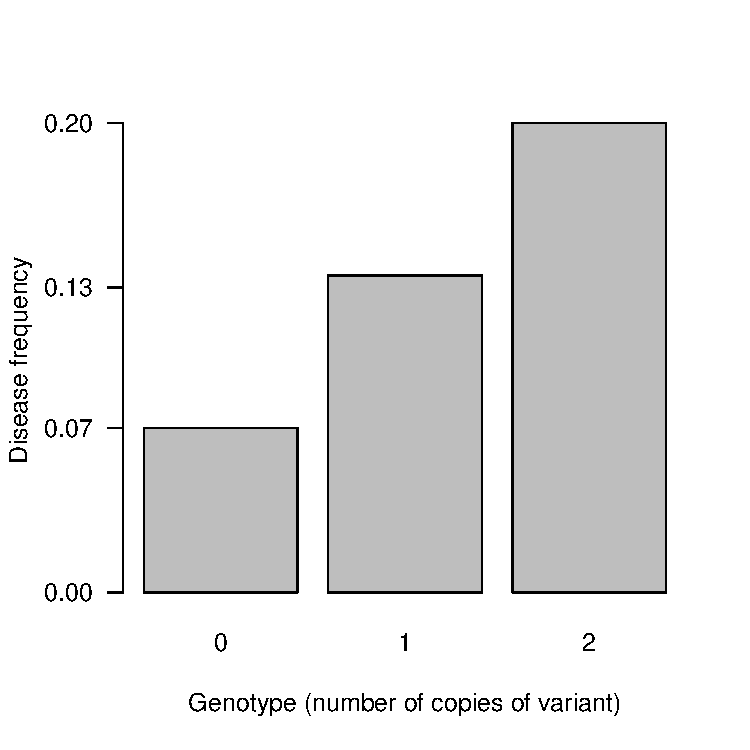
\includegraphics[scale=0.38]{geneticModels7.pdf}\\\vspace{-0cm}
     \item<3-> Rationale: this is what we expect if the variant affects the trait
     \item<4-> Approach: test null hypothesis, $H_0$, of no association (independence)%(low p supports association)
     %\item<4-> Many statistical tests for this can be and are used 
        \end{itemize}
\end{frame}

%%%%
%\begin{frame}
%\frametitle{The simplest tests - genotype based test}
%\vspace{-.7cm}
%\small
%  \begin{itemize}\setlength{\itemindent}{-2.25em}
%   \item Test by applying a $\chi^2$ test to a table w. genotype counts for cases and controls
%   \item I.e. a test w. the test statistic $X^2 = \sum_i \frac{(O_i - E_i)^2}{E_i}$, which is $\sim \chi^2$ under $H_0$
%   \item E.g. assume we have \textbf{observed} this data:
%   \\\vspace{.2cm}
%   \footnotesize
%\hspace{-0.5cm}\begin{tabular}{|l|c|c|c|c|}
%\hline
%  & AA & Aa & aa & Total \\
%\hline
%Case & $O_1$=441 & $O_3$=418 & $O_5$=141 & 1000\\
%\hline
%Control & $O_2$=749 & $O_4$=611 & $O_6$=140 & 1500  \\
%\hline
%Total & 1190 & 1029 & 281 & 2500\\
%\hline
%\end{tabular}\\\vspace{0.2cm}
% \item<2-> \small \textbf{Expected under $H_0$:} if there is no association between the SNP and disease \\\hspace{-0.7cm}we would expect proportions of cases within the genotype categories to be\\\hspace{-0.7cm}the same (here 1000/2500=0.4, i.e. 40\%). 
% \item<3-> \small So e.g. we would expect 40\% of those with genotype AA to be cases and the\\\hspace{-0.7cm}rest to be controls. Thus $E_1$=0.4$\times$1190=476 and $E_2$=1190-476=$714$
%\item<4-> \small \textbf{Small exercise:} what would $E_3$ and $E_4$ be? %similarly we can calculate expected value for the rest of the table and   
%  \end{itemize}
%\end{frame}
\begin{frame}
\frametitle{$\chi^2$ test for independence}
%\vspace{-.7cm}
\small
  \begin{itemize}\setlength{\itemindent}{-2.25em}
   \item A test which you can apply to counts tables for two categorical variables \\
 \hspace{-0.75cm}E.g. disease status and genotypes:   \\\vspace{.2cm}
   \footnotesize
\hspace{-0.5cm}\begin{tabular}{|l|c|c|c|c|}
\hline
  & AA & Aa & aa & Total \\
\hline
Case & 441 & 418 & 141 & 1000\\
\hline
Control & 749 & 611 & 140 & 1500  \\
\hline
Total & 1190 & 1029 & 281 & 2500\\
\hline
\end{tabular}\\\vspace{0.2cm}
  \item<2-> The null hypothesis, $H_0$, of the test, is \textbf{no association} (independence)
  \item<3-> Has the test statistic $X^2 = \sum_i \frac{(O_i - E_i)^2}{E_i}$\\ %, which is $\sim \chi^2$ under $H_0$
    \hspace{-0.75cm}(measures how far your observed data is from what you expect if $H_0$ is true) %the null hypothesis is true   
   \item<4-> If $H_0$ is true then $X^2 \sim \chi^2$ \\
   \hspace{-0.75cm}(This means we can use $\chi^2$ to translate $X^2$ to p-value\\
   \hspace{-0.75cm}i.e. the probability of seeing $\geq X^2$ if $H_0$ is true)
   \item<5-> We use this to decide whether we reject the null hypothesis\\
   \hspace{-0.75cm}(we reject when p is small and see it as evidence for association)\\
 %  (because it means it is not very probably to get $\geq X^2$ if the variables are not associated)       
     \end{itemize}
\end{frame}

%%%%
\begin{frame}
\frametitle{$\chi^2$ tests - test with genotype counts}
\vspace{-.7cm}
\small
  \begin{itemize}\setlength{\itemindent}{-2.25em}
   \item Can be applied to genotype count tables %One So let's try to do this for the count table from before
   \item So assume we have \textbf{observed} this data:
   \\\vspace{.2cm}
   \footnotesize
\hspace{-0.5cm}\begin{tabular}{|l|c|c|c|c|}
\hline
  & AA & Aa & aa & Total \\
\hline
Case & $O_1$=441 & $O_3$=418 & $O_5$=141 & 1000\\
\hline
Control & $O_2$=749 & $O_4$=611 & $O_6$=140 & 1500  \\
\hline
Total & 1190 & 1029 & 281 & 2500\\
\hline
\end{tabular}\\\vspace{0.2cm}
 \item<2-> \small \textbf{Expected under $H_0$:} if there is no association between the SNP and disease \\\hspace{-0.7cm}we would expect proportions of cases within the genotype categories to be\\\hspace{-0.7cm}the same (here 1000/2500=0.4, i.e. 40\%). 
 \item<3-> \small So e.g. we would expect 40\% of those with genotype AA to be cases and the\\\hspace{-0.7cm}rest to be controls. Thus $E_1$=0.4$\times$1190=476 and $E_2$=1190-476=$714$
\item<4-> \small \textbf{Small exercise:} what would $E_3$ and $E_4$ be? %similarly we can calculate expected value for the rest of the table and   
  \end{itemize}
\end{frame}


\begin{frame}
\frametitle{$\chi^2$ tests - test with genotype counts}
\small
\vspace{-0.0cm}
  \begin{itemize}\setlength{\itemindent}{-2.25em}
   \item So we have: \\\vspace{.2cm}
   \footnotesize
\begin{tabular}{|l|c|c|c|c|}
\hline
 \textbf{Observed} & AA & Aa & aa & Total \\
\hline
Case & $O_1$=441 & $O_3$=418\hspace{0.16cm} & $O_5$=141\hspace{0.185cm} & 1000\\
\hline
Control & $O_2$=749 & $O_4$=611\hspace{0.16cm} & $O_6$=140\hspace{0.185cm} & 1500  \\
\hline
Total & 1190 & 1029 & 281 & 2500\\
\hline
\end{tabular}\\\vspace{0.2cm}
 \begin{tabular}{|l|c|c|c|c|}
\hline
 \textbf{Expected} & AA & Aa & aa & Total \\
\hline
Case & $E_1$=476 & $E_3$=411.6 & $E_5$=112.4 & 1000\\
\hline
Control & $E_2$=714 & $E_4$=617.4 & $E_6$=168.6 & 1500  \\
\hline
Total & 1190 & 1029 & 281 & 2500\\
\hline
\end{tabular}
\item<2-> $X^2 = \sum_i \frac{(O_i - E_i)^2}{E_i} = \frac{(441-476)^2}{476}+\frac{(749-714)^2}{714}+... +\frac{(140-168.6)^2}{168.6}$= 16.5838
%\item<2-> \small $X^2$ measures how far the observed counts are from what we would expect if the \\\hspace{-0.7cm}disease is not associated with the SNP (i.e. if $H_0$ is true)
\item<3-> \small Using the $\chi^2$-distribution with 2 df we get a p-value for $X^2$ (p$\simeq$0.00025)%that tells us if this is so far from 0 that is makes us reject the null hypothesis that the SNP is not associated with the disease and conclude they are associated.
\item<4-> \small %p = 0.00025, i.e. 
Tells us that the probability of getting a $X^2$ value 16.5838 or higher \textbf{if} \\\hspace{-0.7cm}there is no association is low (p$\simeq$0.00025$<$0.05)
\item<5-> \small We therefore reject the null hypothesis of no association and conclude that the \\\hspace{-0.7cm}variant is associated with the disease status\\\vspace{0.2cm}\end{itemize}

%Tells us that that the probability of getting a $X^2$ value 16.5838 or higher \textbf{if} \\\hspace{-0.7cm}there is no association is low (p$\simeq$0.00025$<$0.05), suggesting there is association\\\vspace{0.2cm}\end{itemize}
\end{frame}

%\begin{frame}
%\frametitle{$\chi^2$ tests - allelic test}
%\vspace{-.1cm}
%\small
%%\hspace{0.5cm} \includegraphics[scale=.4]{statistics-banner_img.jpg}\\\vspace{0.15cm} 
%  \begin{itemize}
%   \item Often even simpler tests are used, such as the allelic test
%   \item Here we look at count of alleles instead of genotypes, e.g.: % is carried by a case and the same for controls
%  % \item With the previous example:
%    \\\vspace{.2cm}
%   \footnotesize
%\begin{tabular}{|l|c|c|c|c|}
%\hline
% \textbf{Our genotype counts} & AA & Aa & aa & Total \\
%\hline
%Case & 441 & 418\hspace{0.16cm} & 141\hspace{0.185cm} & 1000\\
%\hline
%Control & 749 & 611\hspace{0.16cm} & 140\hspace{0.185cm} & 1500  \\
%\hline
%Total & 1190 & 1029 & 281 & 2500\\
%\hline
%\end{tabular}\\\vspace{0.2cm}
% \begin{tabular}{|l|c|c|c|}
%\hline
% \textbf{Allele counts} & A & a & Total \\
%\hline
%Case &441*2+418=1300 & 418+141*2=700 & 2000\\
%\hline
%Control & 749*2+611=2109 & 611+140*2=891 & 3000\\
%\hline
%Total & 3409& 1591 & 5000\\
%\hline
%\end{tabular}\\\vspace{0.4cm}
%\item \small Otherwise the same as before: we use a $\chi^2$ test %for association %Note this is the example in the book
%\item Main difference is that this test has df=1%Like before we can use a $\chi^2$ test this time with 1 df to test for association
%\item In this case it gives p-value$\simeq$0.00008 and thus also suggests association
%\end{itemize}
%\end{frame}

\begin{frame}
\frametitle{$\chi^2$ tests - specific inheritance models}
\vspace{-.1cm}
\small
%\hspace{0.5cm} \includegraphics[scale=.4]{statistics-banner_img.jpg}\\\vspace{0.15cm} 
  \begin{itemize}
   \item<1-> In a similar way we can test for association \textbf{assuming specific inheritance models} by rewriting the table accordingly and doing a $\chi^2$ test 
   \item<2-> E.g. assuming a \textbf{recessive model} we can rewrite the genotype counts table: % is carried by a case and the same for controls
  % \item With the previous example:
    \\\vspace{.2cm}
   \footnotesize
\begin{tabular}{|l|c|c|c|c|}
\hline
 \textbf{Our genotype counts} & AA & Aa & aa & Total \\
\hline
Case & 441 & 418\hspace{0.16cm} & 141\hspace{0.185cm} & 1000\\
\hline
Control & 749 & 611\hspace{0.16cm} & 140\hspace{0.185cm} & 1500  \\
\hline
Total & 1190 & 1029 & 281 & 2500\\
\hline
\end{tabular}\\\vspace{0.2cm}
\small to\\\vspace{0.2cm}
\footnotesize \begin{tabular}{|l|c|c|c|}
\hline
 \textbf{Counts of homozygous carriers vs others} & AA or Aa & aa & Total \\
\hline
Case &441+418=859 & 141 & 1000\\
\hline
Control & 749+611=1360 & 140 & 1500\\
\hline
Total & 2219 & 281 & 2500\\
\hline
\end{tabular}\\\vspace{0.4cm}
\item<3-> \small Then the same as before: we use a $\chi^2$ test for association w. df=1%Note this is the example in the book
\item<4-> How would you test assuming a dominant model?
%\item Again the test has df=1%Like before we can use a $\chi^2$ test this time with 1 df to test for association
\end{itemize}
\end{frame}

\begin{frame}
\frametitle{Other inheritance models}
\small \vspace{-.25cm}
  \begin{itemize}
\item Commonly considered genetic inheritance models:\\
           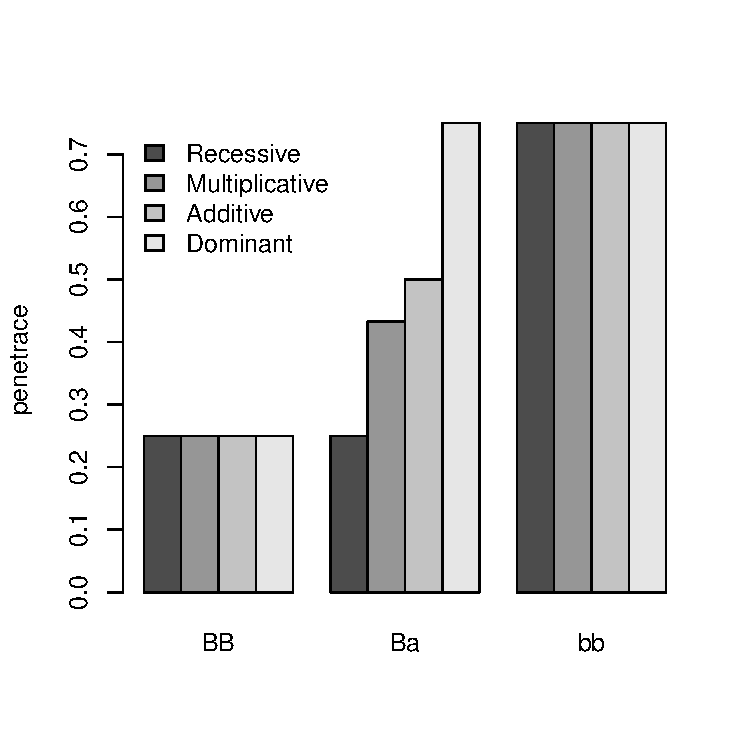
\includegraphics[scale=0.5,trim = 0mm 20mm 0mm 10mm, clip]{geneticModels.pdf}
  \item Testing under an additive genetic inheritance models is more tricky can be done using e.g. an Armitage trend test
  \item Testing under a multiplicative model can be done using logistic regression
  \end{itemize}
\end{frame}


%\begin{frame}
%  \frametitle{Armitage Trend Test}
%  \begin{figure}
%        \includegraphics[scale=0.7]{armitage.png}
% \caption{Is there an additive trend?}
%  \end{figure}
%\end{frame}

%\begin{frame}
%\frametitle{Other inheritance models?}
%\small Other commonly considered genetic inheritance models:\\
%           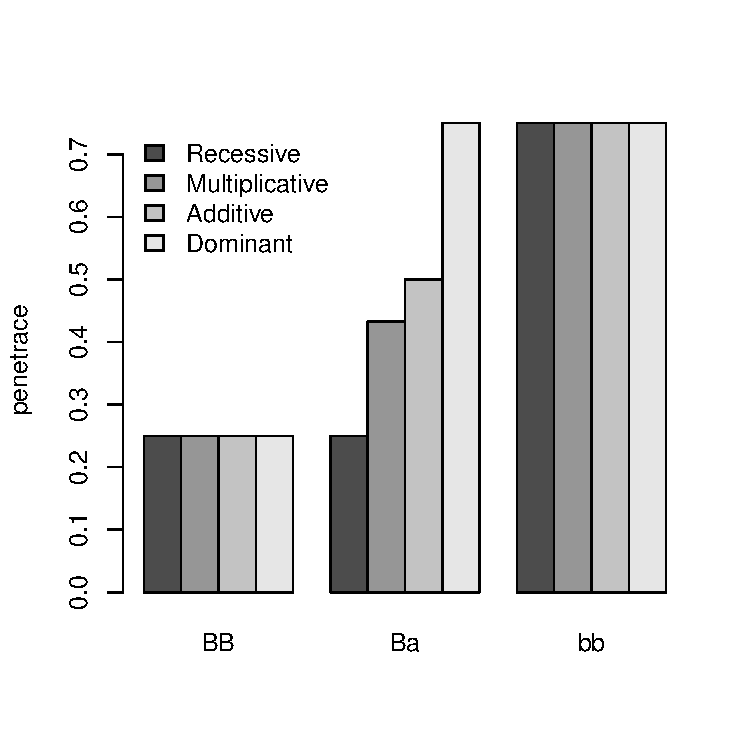
\includegraphics[scale=0.5,trim = 0mm 20mm 0mm 10mm, clip]{geneticModels.pdf}
%  \begin{itemize}
%  \item Can also be tested using tests like the ones we have already talked about 
%  \item And in a logistic regression framework
%  \end{itemize}
%\end{frame}

\begin{frame}
  \frametitle{Logistic regression}
  \small \vspace{-0.7cm}
  \begin{itemize}
  \item<1-> Based on the following general model  
   \[ \log \left(\frac{p_i}{1-p_i}  \right)=\beta_0 +\beta_1x^i_1+\ldots +\beta_nx^i_n\] where the $\beta$s are \emph{regression coefficients} (effect sizes).
   \item<1-> The $x^i$s are determined by the genotype of individual $i$ and the inheritance model 
 \item<2-> E.g. for a simple multiplicative inheritance model we have 
 \[ \log \left(\frac{p_i}{1-p_i}  \right)=\beta_0 +\beta_1x^i_1\]
    where $x^i_1$ is the number number of copies of the variant so 0, 1 or 2%is 1 if $i$ is homozygous carrier of the variant and 0 otherwise
 \item<3-> Test if $\beta_1$ is zero (no association between the variant and the trait) % genotype assuming recessiveness)
     %  \item The $\beta$ covariates are $log$ odds ratios
  \end{itemize}
\end{frame}

%\begin{frame}
%  \frametitle{Other inheritance models (logistic regression)}
%  \vspace{-2cm}
%  \small Most other inheritance models can also be tested by changing the coding of $x^i$: %or different inheritance models 
%  \hspace{-1.5cm}\begin{table}
% \rowcolors{1}{Blue!20}{Blue!5}
%    \begin{tabular}{c|ccccc}
%\hline
%\multicolumn{1}{l}{Genotypes} & \multicolumn{1}{c}{multiplicative} & \multicolumn{1}{c}{dominant} & \multicolumn{1}{c}{recessive} & \multicolumn{2}{c}{genotypes}\\
%\hline
%AA & 0 & 0 & 0 & 0 & 0 \\
%Aa & 1 & 1 & 0 & 1 & 0 \\
%aa & 2 & 1 & 1 & 1 & 1 \\
%\hline
%    \end{tabular}
% %   \caption{covariates ($x$) for genetic models}
%%note that the genotype model has two covariates 
%  \end{table}
%\end{frame}

\begin{frame}
  \frametitle{Why is logistic regression a good framework to use?}
    \vspace{-.3cm}
\small \hspace{0.3cm}Logistic regression is very convenient due to its flexibility:\\\vspace{0.05cm}
 \begin{itemize}
% \item Can be used for different inheritance models
 \item Most inheritance models can be tested (by recoding $x^i$): %or different inheritance models 
 \begin{table}
 \rowcolors{1}{Blue!20}{Blue!5}
    \begin{tabular}{c|ccccc}
\hline
\multicolumn{1}{l}{Genotypes} & \multicolumn{1}{c}{multiplicative} & \multicolumn{1}{c}{dominant} & \multicolumn{1}{c}{recessive} & \multicolumn{2}{c}{genotypes}\\
\hline
AA & 0 & 0 & 0 & 0 & 0 \\
Aa & 1 & 1 & 0 & 1 & 0 \\
aa & 2 & 1 & 1 & 1 & 1 \\
\hline
    \end{tabular}
 %   \caption{covariates ($x$) for genetic models}
%note that the genotype model has two covariates 
  \end{table}
 \item<2-> Can incorporate other factors in the model
   \begin{itemize}
    \item discrete factors such as gender
    \item continuous factors such as age
    \end{itemize}
    Can be used to correct for possible confounding factors\\
    Can be used for metaanalysis by incl a factor for the different studies
%\item Easy to compare nested models using ANOVA
  \end{itemize}
\end{frame}

\begin{frame}
\frametitle{Exercise}
\small
Let's try to perform some of these tests in R:\\\vspace{0.3cm}
Solve exercise 1A, 1B, 1C and 1D (+ 1E if you have time)\\ 
%Purpose: to make you able to have you try perform some of the test in R 
\end{frame}

\subsection{Limitations}
\begin{frame}[fragile]
  \frametitle{Causality?}
  \small 
   \vspace{-.2cm}
  \begin{itemize}
    \item<2-> No, not necessarily!
    \item<3-> We expect to see some loci highly correlated w. causal variant, e.g:\\\vspace{0.2cm}
    %\item I.e. SNP that are highly correlated with a causal SNP, e.g\\\vspace{0.2cm}
    \begin{verbatim}
    Causal     Other locus
    A       	  G
    A       	  G
    A       	  G
    A       	  G
    A       	  G
    C       	  T
    C       	  T
    C       	  T
    \end{verbatim}
    \item<4-> This means that we see association in loci that are in high LD with the causal SNP\\
%    \item<2-> NB LD measure usually used is $r^2$ (ranges 0-1, where 1=fully correlated)  %Means you can test most SNPs using a small subset of SNPs!
So you have to be careful what you conclude from an association signal!
   \end{itemize}
\end{frame}


\begin{frame}[fragile]
  \frametitle{Other important limitations}
  \small 
  % \vspace{-2.2cm}
 One also has to be aware of the underlying assumptions:
 \begin{itemize}%\setlength{\itemindent}{-1.25em}

%    \item<1-> In the allelic test there is an assumption of HWE in the population\\\vspace{0.3cm}\includegraphics[scale=.35]{hwe.png} 
    \item<1-> In all the tests there is an assumption that the individuals are independent (unrelated) and from a homogenous (unstructured) population
    \item<2->  If these assumptions are violated you risk getting false positives!
\item<3-> Hence Quality Control (QC) and appropriate modelling is crucial!
   \end{itemize}
\end{frame}


%\begin{frame}
%  \frametitle{Example}
%\small
%\vspace{-.8cm}
%  \begin{itemize}
%  \item We have 
%    \begin{itemize}
%    \item 2000 cases and 2000 controls
%    \item A disease prevelence of 10\% in the population
%    \item A SNP with minor allele frequency of 0.2
%    \end{itemize}
%  \item We expect a none additive increased disease risk e.g.
%    \begin{itemize}
%    \item Risk is 10\% higher for Aa compared to AA
%    \item Risk is 30\% higher for the aa compared to AA
%    \end{itemize}
%  \item The power to detect an association is
%    \begin{itemize}
%    \item 0.52 for the genotype distribution test
%    \item 0.61 for the allelic count test
%    \end{itemize}
%  \item The wrong model has the most power!
%  \end{itemize}
%\end{frame}


\subsection{Effect sizes}
\begin{frame}
  \frametitle{Effect sizes for case-control data - relative risk}
  \small
\begin{block}{Relative risk - definition}
 % \[OR =\frac{\frac{P(Case|Risk\ genotype\ present)}{P(Control|Risk\ genotype\ present)}}{\frac{P(Case|Risk\ genotype\ absent)}{P(Control|Risk\ genotype\ absent)}} \]\\
 \[RR =\frac{P(Case|Exposed)}{P(Case|Not\ exposed)} \]\\
 where exposed depends on model, e.g. exposed=aa under recessive model \\
\vspace{0.2cm}I.e. how many times higher the \textit{risk} of disease is for exposed\\\vspace{0.1cm}
\end{block}
\begin{block}{Relative risk - example with recessive model}
\vspace{0.1cm}
  {   \rowcolors{1}{Blue!20}{Blue!5}
\scriptsize{
  \begin{table}
\hspace{-2.4cm}    \begin{tabular}{|c|cc|c|}
\hline
      & Cases & Controls & Total \\
\hline
Exposed (g=aa) & 100 & 100 & 200\\
Not exposed (g=AA or Aa) & 400 & 3600 & 4000\\
 \hline   \end{tabular}
      \end{table}
}
}
\vspace{-0.3cm}
\begin{itemize}
\item $P(Case|Exposed) = \frac{100}{200}=  \frac{1}{2}$
\item $P(Case|Not\ exposed) = \frac{400}{4000}= \frac{1}{10}$
\item $RR = \frac{1/2}{1/10} = 5$ 
\end{itemize}
\end{block}
\end{frame}


\begin{frame}
  \frametitle{Effect sizes for case-control data - odds ratio}
  \small
\begin{block}{Odds ratio - definition}
 % \[OR =\frac{\frac{P(Case|Risk\ genotype\ present)}{P(Control|Risk\ genotype\ present)}}{\frac{P(Case|Risk\ genotype\ absent)}{P(Control|Risk\ genotype\ absent)}} \]\\
 \[OR =\frac{ODD_{Exposed}}{ODD_{Not\ Exposed}}=\frac{\frac{P(Case|Exposed)}{P(Control|Exposed)}}{\frac{P(Case|Not\ exposed)}{P(Control|Not\ exposed)}} \]\\
 where exposed depends on model, e.g. exposed=aa under recessive model \\
\vspace{0.2cm}I.e. how many times higher the \textit{odds} of disease is for exposed\\\vspace{0.1cm}
\end{block}
\begin{block}{Odds ratio - example with recessive model}
\vspace{0.1cm}
  {   \rowcolors{1}{Blue!20}{Blue!5}
\scriptsize{
  \begin{table}
\hspace{-2.4cm}    \begin{tabular}{|c|cc|c|}
\hline
      & Cases & Controls & Total \\
\hline
Exposed (g=aa) & 100 & 100 & 200\\
Not exposed (g=AA or Aa) & 400 & 3600 & 4000\\
 \hline   \end{tabular}
      \end{table}
}
}
\vspace{-0.3cm}
\begin{itemize}
\item $\frac{P(Case|Exposed)}{P(Control|Exposed)} = \frac{100/200}{100/200}=  \frac{100}{100}=1$
\item $\frac{P(Case|Not\ exposed)}{P(Control|Not\ exposed)} = \frac{400/4000}{3600/4000}= \frac{400}{3600}=1/9$
\item $OR = \frac{1}{1/9} = 9$ (very high for an association study!)
\end{itemize}
\end{block}
\end{frame}

\begin{frame}
  \frametitle{Effect size estimates from logistic regression}
\vspace{-1.4cm}\small
\begin{itemize}
  \item<1-> In logistic regression the ORs are estimated directly:\\ 
  In the model we estimate the effect size $\beta_1$
     \[ \log \left(\frac{p_i}{1-p_i}  \right)=\beta_0 +\beta_1x^i_1 \dots \] 
\item<2-> Example: recessive model
    \[ \frac{\text{ODD}_{aa}}{\text{ODD}_{aA/AA}} = \frac{ \frac{p_{aa}}{1-p_{aa}} }{\frac{p_{aA/AA}}{1-p_{aA/AA}} } =\frac{\exp(\beta_0 +\beta_1)}{\exp(\beta_0)} = \exp(\beta_1) \] 
\item<3-> So we can get OR by taking the exp() of $\beta_1$
\item<4-> If time allows do exercise 1F  
\end{itemize}
\end{frame}


\subsection{Design}
\begin{frame}
%\vspace{-.9cm}
  \frametitle{Design}
\small 
%\vspace{-.3cm}
%\hspace{0.5cm}   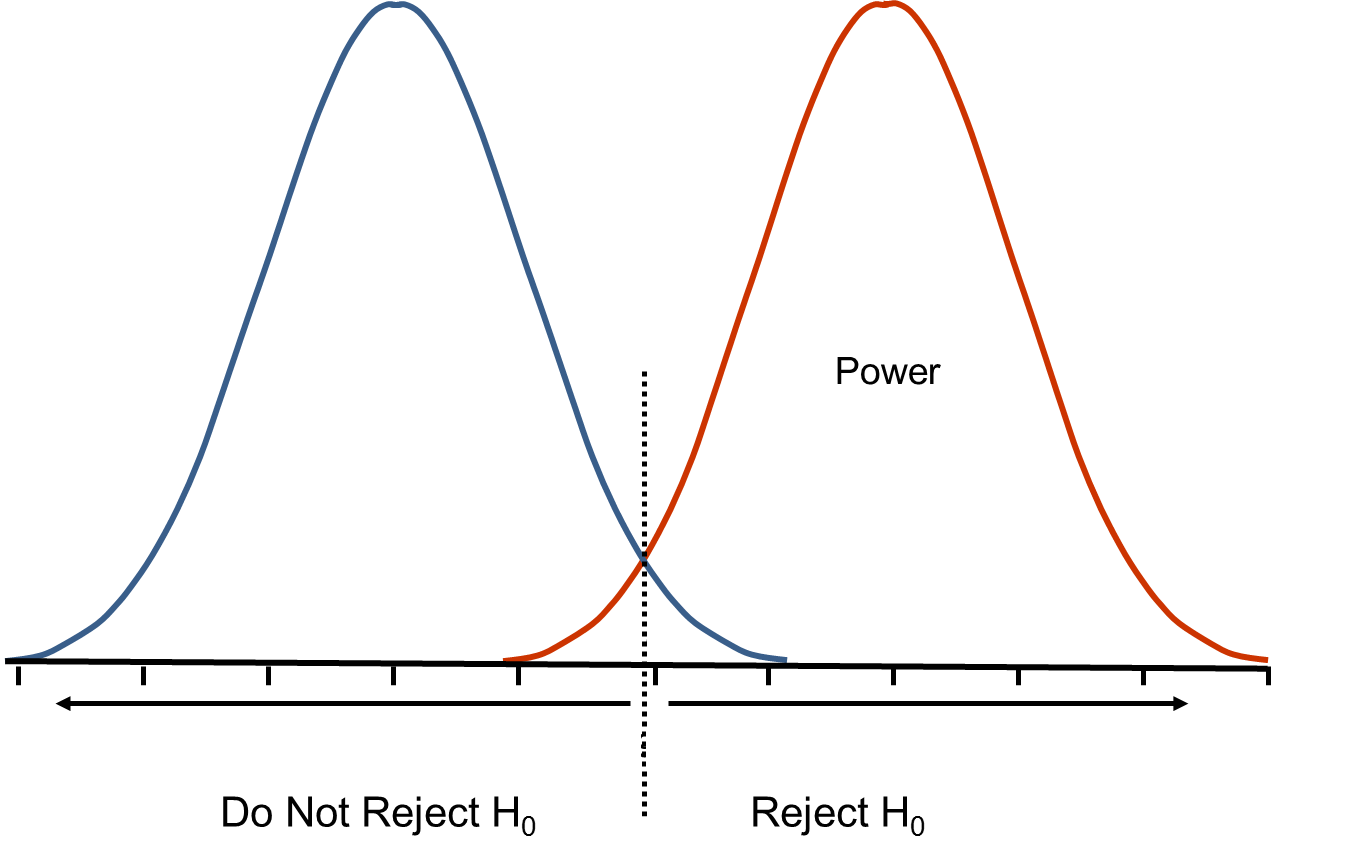
\includegraphics[scale=.2]{RejectionRegion3b.png}\\\vspace{0.05cm}
  \begin{itemize}
 \item<1-> Will your study answer your research question? \textbf{Key: power}
 \item<2-> Power is the probability that a true association is found when testing\\\vspace{0.3cm}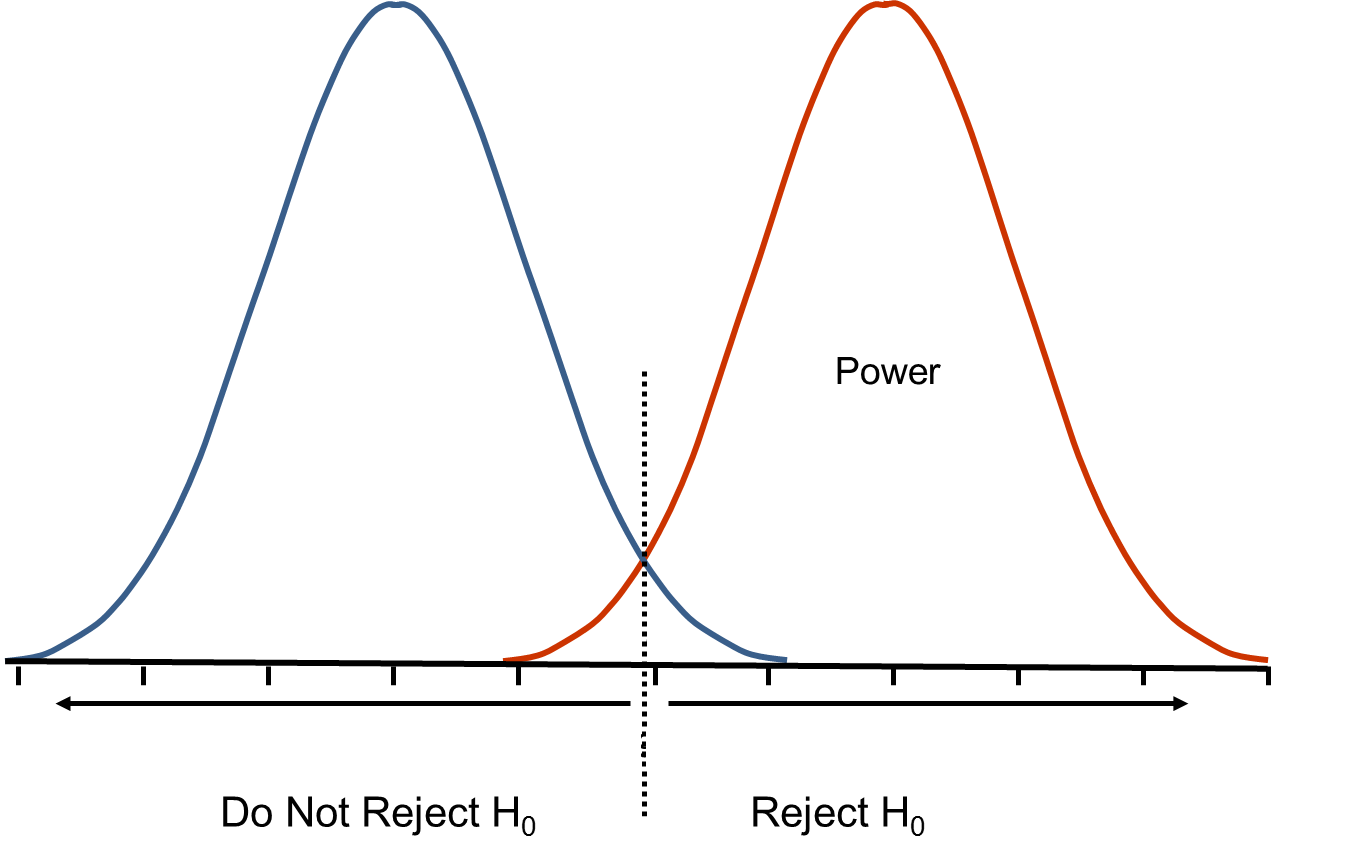
\includegraphics[scale=.25]{RejectionRegion3b.png}\\\vspace{0.05cm}
Crucial for whether the study is worth performing!% If power is low then it is not worth performing the study!
\item<3-> Before you start your study: calculate power for your study and assess it
 Rule of thumb: power should be at least 0.8 
    \end{itemize}
\end{frame}

\begin{frame}
\vspace{-.8cm}
  \frametitle{Power and power calculations}
  \small
  \begin{itemize}
 \item<1-> Power depends on
 \begin{itemize}
  \item the inheritance mode, e.g. recessive effect
   \item the effect size, e.g. OR of 1.3 (the bigger the higher power)
    \item the frequency of allele, e.g. 0.04 (the bigger the higher power)
  \item \textbf{the rejection criterion}, e.g. $p<0.05$ (the bigger the higher power)
  \item \textbf{the number of samples} (the bigger the higher power) 
 \item \textbf{the test you use} 
   \end{itemize}
\item<2-> Can often be calculated using "power-calculators"
 \item<3-> So before you start: \\Do power calculations to make sure you will have enough samples!
 \item<4-> To detect association we might not choose the model that is most correct, but instead choose the model that has the most power
    \end{itemize}
\end{frame}

\section{Quantitative traits}
\begin{frame}
 \frametitle{Quantitative trait}
  \begin{itemize}
 \item<1-> Distribution of the trait in the population\\\vspace{-0.3cm}
 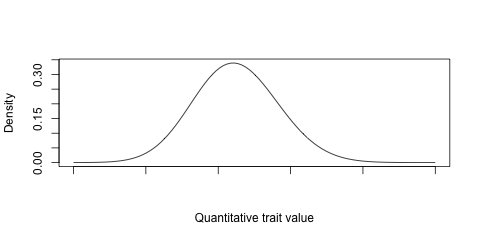
\includegraphics[scale=.4]{qtl_dist_pop.png}
  \item<2-> If a variant influence the trait value, we expect:\\\vspace{-0.3cm}
   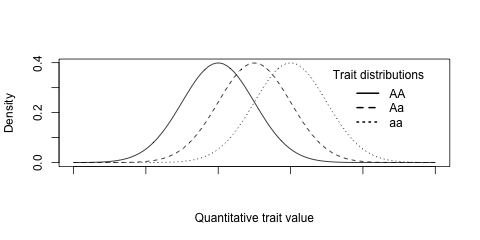
\includegraphics[scale=.4]{qtl_dist.png}
  % \item<1-> Distribution of trait in the population
\end{itemize} 
\end{frame}

\begin{frame}
  \frametitle{Linear regression}
  \small \vspace{-0.7cm}
  \begin{itemize}
  \item<1-> Based on the following general model  
   \[ \text{E}(y_i) = \beta_0 +\beta_1x^i_1+\ldots +\beta_nx^i_n\] where the $\beta$s are \emph{regression coefficients} (effect sizes).
   \item<1-> The $x^i$s are determined by the genotype of individual $i$ and the inheritance model 
 \item<2-> E.g. for a simple additive inheritance model we have 
 \[ \text{E}(y_i) = \beta_0 +\beta_1x^i_1\]
    where $x^i_1$ is the number number of copies of the variant so 0, 1 or 2
 \item<3-> Test if $\beta_1$ is zero (no association between the variant and the trait) 
  \end{itemize}
\end{frame}


\section{Genome-Wide Association Studies (GWASs)}

\subsection{Introduction to GWAS}
\begin{frame}
  \frametitle{Types of association studies}
  \vspace{-1cm}
  \begin{itemize}
  \item<1-> Candidate causative genetic variant
 \begin{itemize}
 \item 
1 SNP or deletion, duplication.
Evidence from other study
\end{itemize}
\item<1-> Candidate causative gene 
 \begin{itemize}
 \item 5-50 SNPs.
Evidence from other study or function\end{itemize}

\item<1-> 
Candidate causative region \begin{itemize}
\item<1->
100s of SNPs
Evidence from other study\end{itemize}

\item<1-> 
Genome-wide (GWAS) \begin{itemize}
\item<1-> 
$>$500,000 SNPs.
No prior evidence required
\end{itemize}
  \end{itemize}
\end{frame}

\begin{frame}
  \frametitle{Why GWAS?}
\vspace{-.1cm}
  \small 
    \begin{itemize}\setlength{\itemindent}{-1.5em}
    \item If we look at 500.000 SNPs we are likely not to have the causal SNP!\\\vspace{0.2cm}
    \item But, remember SNPs in high LD with a causal SNP will also be associated: \\ \vspace{0.3cm}       
      \hspace{1cm} 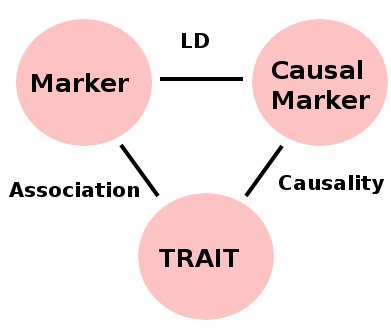
\includegraphics[scale=.35,trim = 0mm 0mm 0mm 0mm, clip]{asso.png}\\\vspace{0.15cm}
      
     \end{itemize}  
\end{frame}

\begin{frame}
  \frametitle{Why GWAS?}
\vspace{-.1cm}
    \begin{itemize}
    \item SNPs are in high LD in blocks along the human genome\\\vspace{0.2cm}
            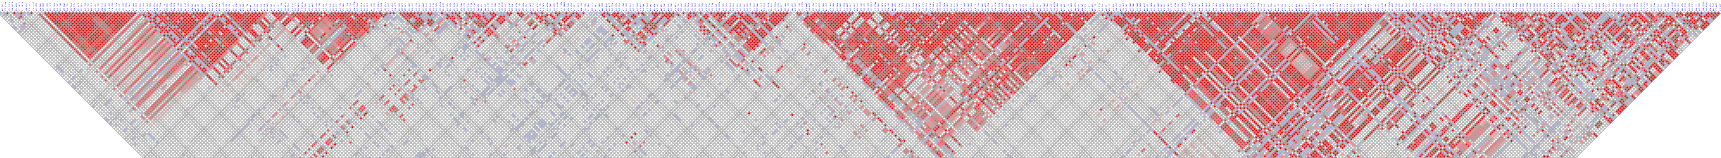
\includegraphics[scale=.16]{ldBlock.png}\\\vspace{0.15cm}
        %  \includegraphics[scale=.18]{linkage_disequilibrium_maps.png}\\\vspace{0.15cm}
        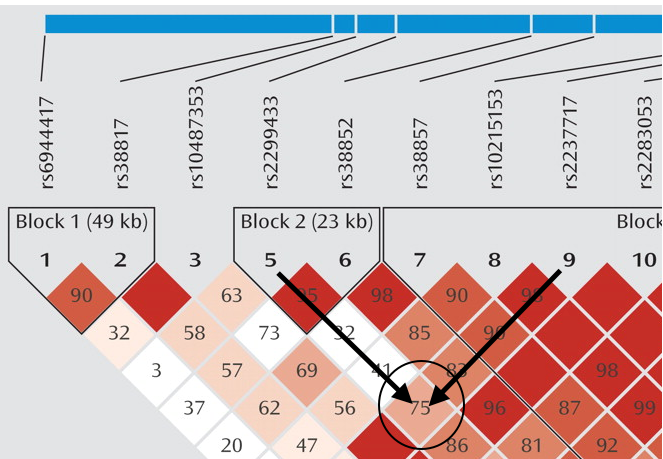
\includegraphics[scale=.24,trim = 0mm 0mm 0mm 30mm, clip]{reading_LD_blocks.png}\\\vspace{0.15cm}
       \end{itemize}  
\end{frame}


\begin{frame}
  \frametitle{Why GWAS?}
\vspace{-.1cm}
    \begin{itemize}
          \item<1-> By testing a few SNPs in each block most common SNPs are indirectly tested
   %\item<2-> Also holds genome-wide! (so the causal SNP does not need to be typed)
   \item<2-> We can test most common SNPs (indirectly) by using $\geq500,000$ SNPs
   \item<3-> Pro: Cheap! (only need to genotype $\geq500,000$ SNPs) \\
   Con: We are far from sure the identified SNPs (if any) are causal!  
       \end{itemize}  
\end{frame}

\begin{frame}
  \frametitle{When GWAS?}
\vspace{-.1cm}
  \small 
    \begin{figure}
      \scalebox{0.70} {
        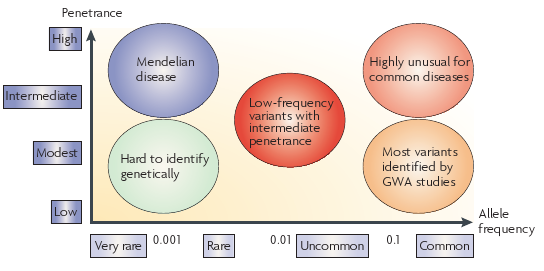
\includegraphics{AssoTypes.png}
      }
\caption{Strategies for locating disease loci}
  \end{figure}
\end{frame}

\subsection{How to perform a GWAS}
\begin{frame}
\vspace{-.5cm}
  \frametitle{How GWAS (step-by-step overview)}
 \small 
  \begin{enumerate}
 \item Collect samples and traits of interest (based on power calculations!)%, e.g 5000 cases and 5000 controls
  \item Genotype samples at a number of SNP loci ($\geq$500,000) 
  \item Lots and lots of quality control (QC)!
  \item Statistically test each SNP for association
%  \item Assess the distribution of association and identify candidates
\item Assess the results: 
\begin{itemize}
\item make sure things went OK 
\item identify associated SNPs
    \end{itemize}  
\item	Identify causal variant (if possible)
\item	Replicate associations in a different dataset
\item Investigate what the underlying biological mechanism is
\item Ideal longterm goal/hope: better prevention or treatment
  \end{enumerate}
\end{frame}

\begin{frame}
\vspace{-.5cm}
  \frametitle{GWAS step-by-step}
 \small 
  \begin{enumerate}
 \item Collect samples and traits of interest (based on power calculations!) %, e.g 5000 cases and 5000 controls
  \item Genotype samples at a number ($\geq$500,000) of SNP loci 
  \item \textbf{Lots and lots of quality control (QC)!}
  \item \textbf{Statistically test each SNP for association}
\item \textbf{Assess the results:} 
\begin{itemize}
\item \textbf{make sure things went OK} 
\item \textbf{identify associated SNPs}
    \end{itemize}  
\item	Identify causal variant (if possible)
\item	Replicate associations in a different dataset
\item Investigate what the underlying biological mechanism is
\item Ideal longterm goal/hope: better prevention or treatment
  \end{enumerate}
\end{frame}

%\subsection{Statistically test each SNP for association}
\begin{frame}
  \frametitle{Statistically test each SNP for association}
\small
\vspace{-2.8cm}
\begin{itemize}
\item Use one of the tests you just learned how to perform
\item There are programs like PLINK2 that will help you do this 
\item Can be done using one 1-line command 
\item Also offers functions for doing QC (we'll see that later)
\end{itemize}
\end{frame}

\subsection{Assessing results}
\begin{frame}
  \frametitle{Identify associated SNPs}
\begin{block}{Manhattan plot}
   \vspace{0.4cm}
    
      \scalebox{0.42} {
        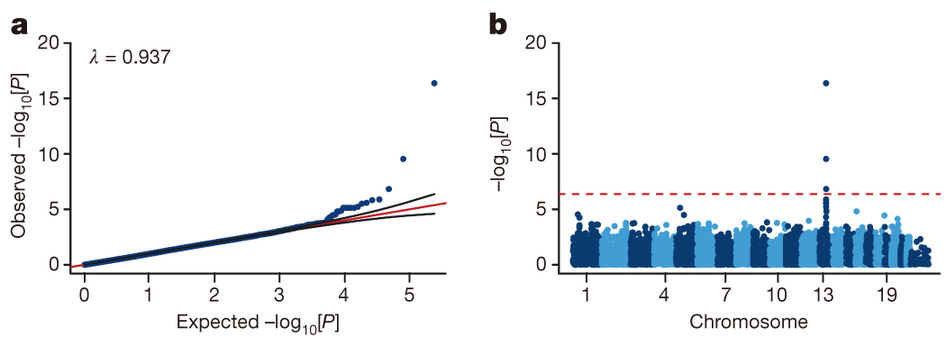
\includegraphics[trim = 170mm 0mm 0mm 12.5mm, clip]{nature13425-f2.jpg}
      }
\end{block}
\end{frame}

\begin{frame}
  \frametitle{What p-value threshold to use}
\small
\begin{itemize}
\item<1-> Usually for a single test we use a p-value threshold of $\alpha=0.05$ 
\item<2-> If you perform many tests w. this $\alpha$ some will be falsely rejected\\
With threshold 0.05 thousands of false positives!! (-log(0.05)=1.3)\\
\vspace{0.2cm}
 \scalebox{0.32} {
        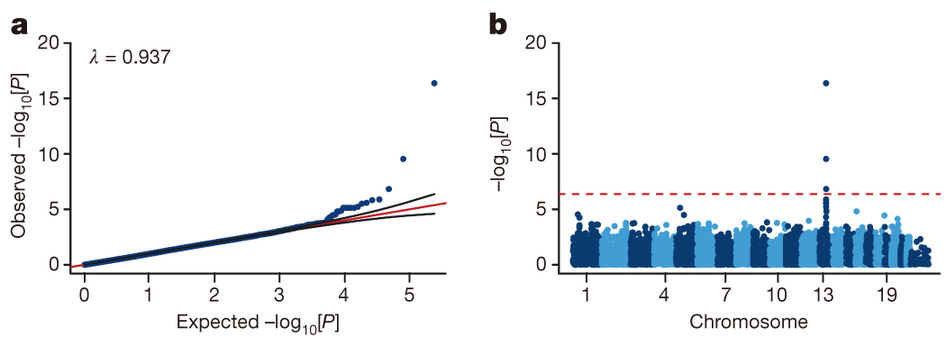
\includegraphics[trim = 170mm 10mm 0mm 12.5mm, clip]{nature13425-f2.jpg}
      }   \\
    So we have to \textbf{correct for multiple testing}
    \item<3-> Often \textbf{Bonferroni correction} is used; $\alpha$ is divided by the number of tests: 
      \begin{itemize}
      \item E.g. 100000 SNPs and $\alpha=0.05$
      \item Bonferroni corrected $\alpha =0.05/100000=0.0000005 = 5\times10^{-7}$ 
      \item Which on the Manhattan plot is $-log_{10}(5\times10^{-7})=6.3$
      \end{itemize}
%   \item<2-> Often $5\times10^{-8}$ is used (so $-log_{10}(p)$ threshold of 7.3)
\end{itemize}
\end{frame}

\begin{frame}
  \frametitle{Exercise}
  Solve exercise 2A, i.e. perform your first GWAS analysis :)
\end{frame}


\begin{frame}
  \frametitle{Make sure things went OK!}
\begin{block}{QQ-plots and genomic control inflation factor $\lambda$}
  %  \begin{figure}
      \vspace{0.4cm}
      \scalebox{0.42} {
        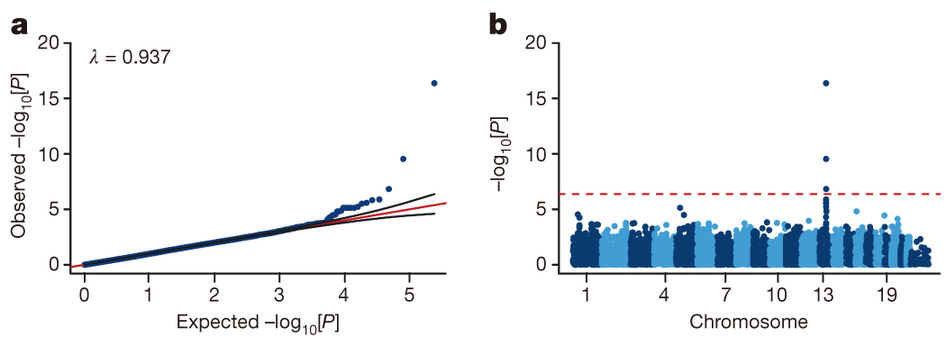
\includegraphics[trim = 0mm 0mm 170mm 12.55mm, clip]{nature13425-f2.jpg}   
      }\\\vspace{0.2cm}
%\end{figure}
\textbf{If so most of the dots will be on the x=y line and $\lambda\simeq1$}
\end{block}

\end{frame}

\begin{frame}
  \frametitle{Exercise}
  \small Solve exercise 2B, i.e. check if your results look OK...
\end{frame}

\subsection{Lots and lots of QC}

\begin{frame}
\frametitle{Lots and lots of QC}
\vspace{-.9cm}
\small
This shows why we usually do QC first ...! :)\\\vspace{0.2cm}
Let's therefore return to that step\\
(we wont go through all QCs, but some important ones)
\end{frame}

\begin{frame}
\frametitle{Sample mislabling?}
\vspace{-1.9cm}
\small
\begin{itemize}
\item One thing that can go wrong is the samples can be misslabled
\item If so, genotypes won't match phenotypes
\item This is difficult to catch
\item But a simple check is to see of gender is correct
\item If not the disease status is likely not to be either...
\item We can check this using PLINK2
\item<2-> \textbf{Exercise:} try checking it for your data (exercise 2C)
\end{itemize}

\end{frame}

\begin{frame}
\frametitle{Closely related individuals or duplicates?}
\vspace{-1.9cm}
\small
\begin{itemize}
\item All association tests mentioned assume that the participants are \textbf{independent} samples from a population
\item This would not be the case if some participants 
\begin{itemize}
\item are closely related 
\item represented more than once 
\end{itemize}
\item One way to check if this is the case is to use PLINK2 (again) % can check this is to if this is violated by using PLINK to estimate if the samples are closely related
%\item We can check this using PLINK
\item<2-> \textbf{Exercise:} try checking it for your data (exercise 2D)
\end{itemize}

\end{frame}

\begin{frame}
\frametitle{Batch biases/non-random genotyping error?}
\vspace{-1.9cm}
\small
\begin{itemize}
\item Sometimes the data handling/generation process can lead to non-random genotyping errors
\item E.g. if all cases were genotyped first and then all controls, then changes in genotyping procedure along the way may lead to non-random differences in genotypes between cases and controls    
\item  This may lead the false positive association test results
\item<2-> \textbf{Exercise:} try checking it for your data (exercise 2E+F if there is time)
\end{itemize}
\end{frame}

\begin{frame}
\frametitle{Additional important checks?}
\vspace{-2.4cm}
\small
\begin{itemize}
\item Other additional signs of something being wrong include:
\begin{itemize}
\item high missingness in specific loci/individuals   
\item loci (strongly) out of Hardy-Weinberg Equilibrium (why?)
\end{itemize}
\item Furthermore, low frequency variants tend to be difficult to genotype
\item Removing such loci/individuals can help a lot
\item<2-> \textbf{Exercise:} try rerunning your analyses with these QC filters (exercise 2G)% if there is time)
\end{itemize}
\end{frame}


\subsection{GWAS perspectives (if time allows)}
\begin{frame}
  \frametitle{First study went extremely well!}
\begin{itemize}
\item Study of age-related Macular Degeneration (Klein et al. 2005)
% major cause of blindness in the elderl
\item 96 cases and 50 controls, 100K SNPs\\\vspace{0.2cm}
    \begin{figure}\scalebox{0.4}{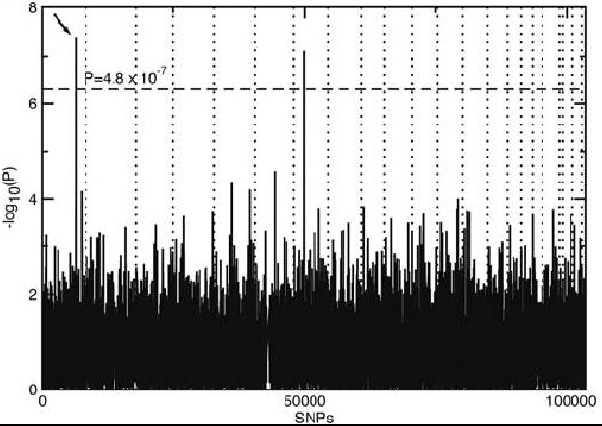
\includegraphics[trim = 0mm 0mm 0mm 6mm, clip]{eye}}\end{figure}    
\item SNP in \textit{CFH} w large effect (OR=7.4)+led to new biological insight 
\end{itemize} % in an intron of \textit{CFH} on 1q31
\end{frame}

\begin{frame}
  \frametitle{Turned out to be unusual...}
\begin{itemize}
\item MANY studies and many associations%\\\vspace{0.2cm}
\item But in the beginning few were replicated\\(underpowered, population structure, insufficient corr. for multiple tests)
%  \begin{figure}\scalebox{0.5}{\includegraphics[trim = 0mm 0mm 0mm 6mm, clip]{gwas3}}\end{figure}    
\item So later studies have many more samples and are much stricter 
\item And most found small effect sizes and limited biological insight
%\item<2-> E.g. Voight et al. (2010) in Nature Genetics :\\\vspace{.1cm}
  %\includegraphics[scale=0.35,trim = 0mm 50mm 0mm 90mm, clip]{T2Dgwas.png} \\ 
%\begin{itemize}
%\item About 8000 cases and 39000 controls\\	
%\item OR of at most 1.4 for GWAS of T2D among Europeans\\
%\item And led to very limited biological insights
%\end{itemize}
\end{itemize}
\end{frame}


%\begin{frame}
%  \frametitle{Example of a wrong model with more power}
%\small
%\vspace{-.8cm}
%  \begin{itemize}
%  \item We have 
%    \begin{itemize}
%    \item 2000 cases and 2000 controls
%    \item A disease prevelence of 10\% in the population
%    \item A SNP with minor allele frequency of 0.2
%    \end{itemize}
%  \item We expect a none additive increased disease risk e.g.
%    \begin{itemize}
%    \item Risk is 10\% higher for Aa compared to AA
%    \item Risk is 30\% higher for the aa compared to AA
%    \end{itemize}
%  \item The power to detect an association is
%    \begin{itemize}
%    \item 0.52 for the genotype distribution test
%    \item 0.61 for the allelic count test
%    \end{itemize}
%  \item The wrong model has the most power!
%  \end{itemize}
%\end{frame}


\begin{frame}
  \frametitle{NGS enters the stage}
\begin{itemize}
\item Reference panels
\begin{itemize}
\item 1000 genomes project
\item Haplotype reference consortium
\end{itemize}
\item Imputation:
\item[] 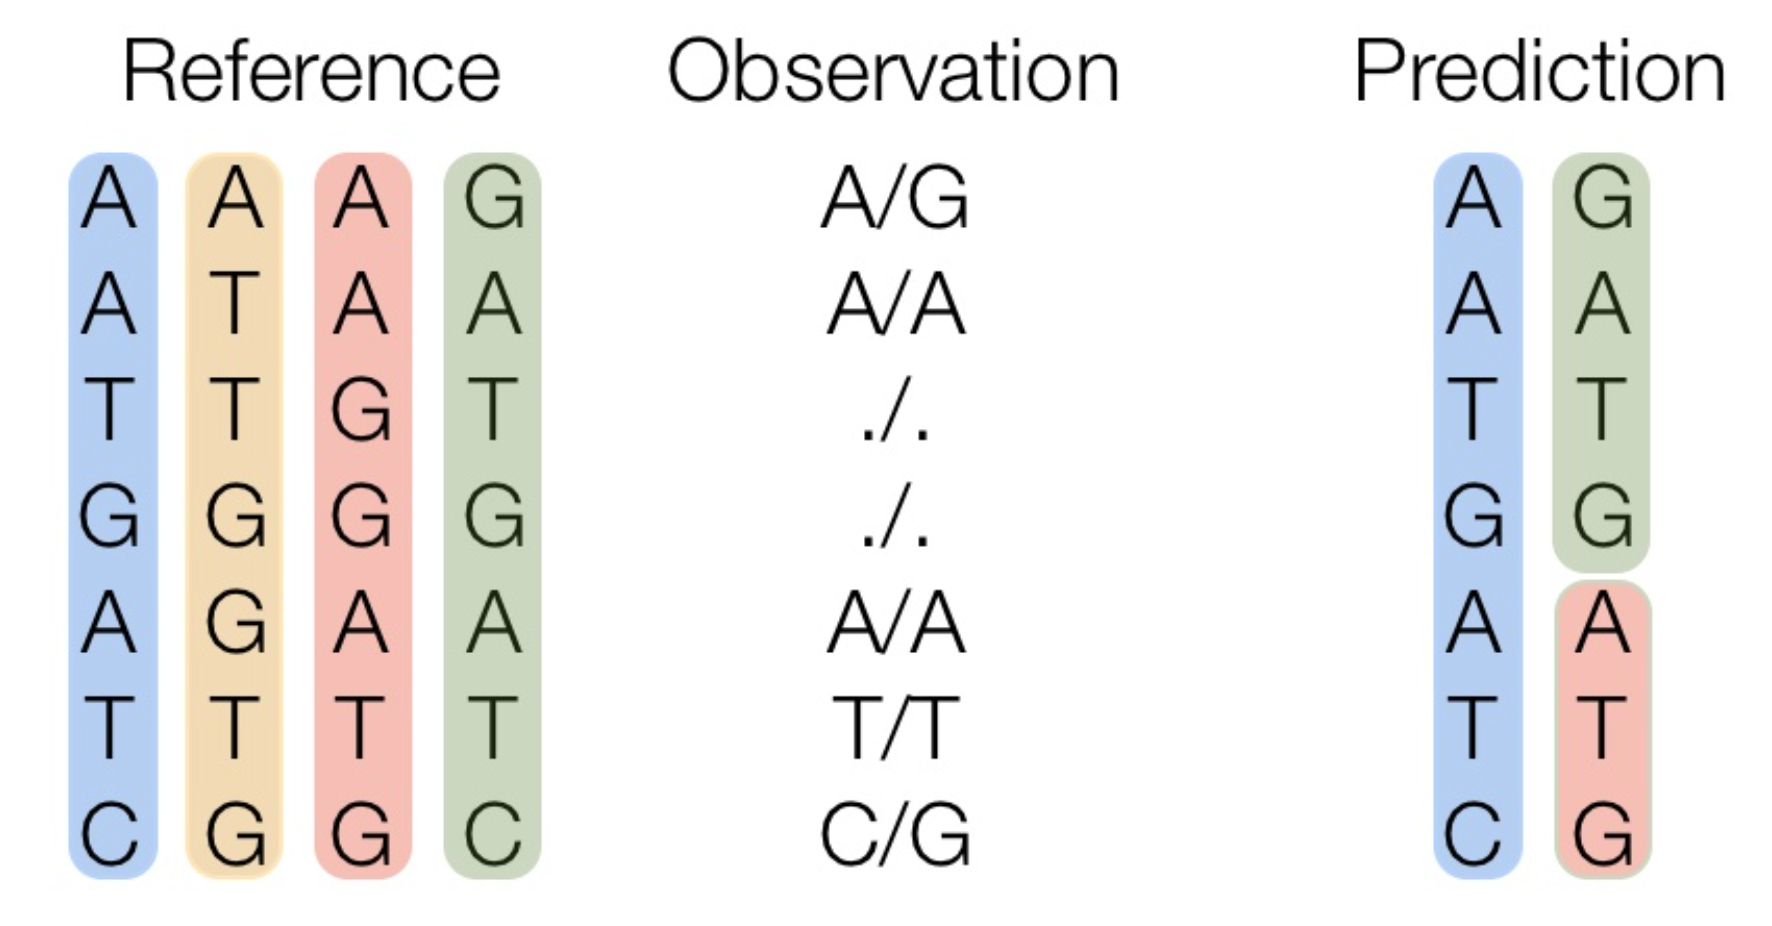
\includegraphics[width=0.6\textwidth]{imputation_illustration.png} 
\item Results in posterior genotype probabilities. 
\end{itemize}
\end{frame}


\begin{frame}
  \frametitle{Dealing with uncertain genotypes in associations}
\begin{itemize}
\item The easy solution: DOSAGE

 $$E[g] = \sum_{g=0}^{2}g\ p(G=g | X)$$

\item The complicated solution: Full likelihood model
$$p(y | X) = \prod_{i} \sum_{g} p(y_i | G_i =g)p(G_i = g | X_i)$$

\item Same goes for association studies based on directly on sequencing data.
\end{itemize}
\end{frame}



\end{document}
 
 

% LocalWords:  quantiles